\chapter{Balanced Detection}
\label{appendix:RIN}
% Referenced from: Sec 2.6, Table 3.1 (balanced-detection row), Sec 5.1.3 and
% Sec 5.2.3 (via \autoref{eq:beat_power}).
As discussed  in \autoref{sec:lit-noiseSources}, the best-case performance of a DWL system is for it to operate in a shot-noise limited regime - thus, all other sources of noise should be reduced to below the shot-noise level. In coherent detection LiDAR architectures, the use of a balanced detector setup has become common for this purpose, as it assists in reducing a laser source's relative-intensity noise (RIN) below the shot-noise level, in a manner which single-ended detection does not.

A single-ended detection system simply uses a 2:1 (2 inputs, one output) fiber optic coupler to mix the LO reference signal with the backscatter signal, and uses a single photodetector to convert this light signal into a measurable current. It can be seen that this detection method retains the DC terms $P_{LO}$, $P_{RS}$. Any RIN from the laser source is present in the output, as these intensity fluctuations are contained in these two power terms. Thus, the measurable Doppler peak will be smaller with respect to the noise floor.

Contrastingly, balanced detection setup makes use of a 2:2 fibre optic coupler which also optically mixes the LO reference signal with the received backscatter signal (as discussed in \autoref{sec:lit-coherentDetection}). However, the 2:2 coupler has two outputs, thus giving two output signals which can be termed $E_1$ and $E_2$ \cite{kikuchi_fundamentals_2016}:

\begin{equation}
	E_1 = \frac{1}{\sqrt2}(E_{RS} + E_{LO}), \space
	E_2 = \frac{1}{\sqrt{2}}(E_{RS} - E_{LO})
\end{equation}
Where $E_{RS}$ and $E_{LO}$ are the complex electromagnetic fields of the returned backscatter signal and the local oscillator respectively.

Thereafter, the two signals enter the balanced detector, which consists of two matched photodiodes and a transimpedance amplifier to convert their currents into a measurable voltage. The photodiodes respond with currents $I_1$ and $I_2$ respectively, proportional to the intensity of the electromagnetic field incident on it ($|E_{1}|^2$ and $|E_2|^2$ respectively), as was also discussed in \autoref{sec:lit-coherentDetection}. Due to the internal setup of the transimpedance amplifier and the photodiodes in the balanced detector, the output current is then given by \cite{kikuchi_fundamentals_2016}:

\begin{equation}
	I_{det} \propto I_1 - I_2 \propto |E_1|^2 - |E_2|^2 \newline
	\propto 2\sqrt{P_{LO}P_{RS}} cos(2\pi\Delta f t)
\end{equation}

Comparing this to \autoref{eqn:beatSignal}, it can be seen that the DC terms $P_{LO}$ and $P_{RS}$ are no longer present due to them being common-mode in both $I_1$ and $I_2$ and thus being canceled by the subtraction. This therefore lowers the noise floor, as the RIN contained in these terms is also eliminated.

Writing in the photodiode responsivity $R$ and the transimpedance gain $G$ of
the balanced detector, the output voltage of the detector is
\begin{equation}
	V(t) = G\,(I_1 - I_2) = 2GR\sqrt{P_{LO}P_{RS}}\,\cos(2\pi\Delta f\,t),
	\label{eq:beat_voltage}
\end{equation}
where $P_{LO}$ and $P_{RS}$ are the total LO and received powers entering the
coupler.

It must also be noted that since the mean of $\cos^2$ is $\tfrac{1}{2}$, the mean-square voltage of the beat signal is
\begin{equation}
	\langle V^2 \rangle = 2G^2R^2P_{LO}P_{RS}.
	\label{eq:beat_power}
\end{equation}
Thus, by Parseval's theorem, $\langle V^2 \rangle$ equals the PSD integrated across
the Doppler peak, so a measured excess power can allow one to estimate the received signal power:
$P_{RS} = \langle V^2 \rangle / (2G^2R^2P_{LO})$.


\autoref{fig:balanceddetector} depicts the balanced detection process graphically:
\begin{figure}[H]
	\centering
	\begin{tikzpicture}[font=\small, line width=0.7pt]

		% ---- inputs ----
		\draw[->] (0.3,2.25) -- (2.2,2.25);
		\node[above] at (1.25,2.25) {$E_{LO}$ (LO)};
		\draw[->] (0.3,0.75) -- (2.2,0.75);
		\node[below, align=center] at (1.25,0.75) {$E_{RS}$\\(backscatter)};

		% ---- coupler ----
		\draw[rounded corners=2pt] (2.2,0.25) rectangle (4.0,2.75);
		\node[align=center] at (3.1,1.5) {50:50\\coupler};

		% ---- coupler outputs ----
		\draw[->] (4.0,2.25) -- (9.0,2.25);
		\node[above] at (6.5,2.25) {$E_1 = \tfrac{1}{\sqrt{2}}(E_{RS} + E_{LO})$};
		\draw[->] (4.0,0.75) -- (9.0,0.75);
		\node[below] at (6.5,0.75) {$E_2 = \tfrac{1}{\sqrt{2}}(E_{RS} - E_{LO})$};

		% ---- balanced detector ----
		\draw[rounded corners=2pt] (9.0,-0.25) rectangle (12.0,3.25);
		\node[above] at (10.5,3.25) {Balanced detector};
		\draw[rounded corners=1pt] (9.3,1.85) rectangle (10.5,2.65);
		\node at (9.9,2.25) {PD$_1$};
		\draw[rounded corners=1pt] (9.3,0.35) rectangle (10.5,1.15);
		\node at (9.9,0.75) {PD$_2$};

		% ---- difference ----
		\draw (10.5,2.25) -- (11.0,2.25) -- (11.0,0.75) -- (10.5,0.75);
		\node[above, font=\footnotesize] at (10.75,2.25) {$I_1$};
		\node[below, font=\footnotesize] at (10.75,0.75) {$I_2$};
		\fill (11.0,1.5) circle (1.5pt);
		\draw (11.0,1.5) -- (12.0,1.5);

		% ---- output ----
		\draw[->] (12.0,1.5) -- (12.7,1.5);
		\node[right] at (12.7,1.5) {$I_1 - I_2$};
	\end{tikzpicture}
	\caption{Balanced detection. The 50:50 coupler delivers the sum and difference
		of the backscatter and LO fields to two matched photodiodes; the output is the
		difference of their photocurrents, in which the common-mode terms cancel and
		only the beat term $2\sqrt{P_{LO} P_{RS}}\cos(2\pi\Delta f t)$ remains.}
	\label{fig:balanceddetector}
\end{figure}

It can thus be seen that balanced detection provides the advantage of cancelling RIN. This allows for the final detected signal to theoretically be able to achieve the desired shot-noise limited operation (if other sources of noise are also eliminated).
